\documentclass[]{../template/Report}%方括号内写yuxi即生成预习报告\documentclass[yuxi]{../template/Report}
\settemplatedir{../template/}%设置模板路径

\exname{惠斯登电桥} %实验名称
\extable{8} %实验桌号
\instructor{宋斌} %指导教师
\class{信工2401} %班级
\name{姚舜瑜} %姓名
\stuid{3240100532} %学号

\nyear{2025} %年
\nmonth{10} %月
\nday{14} %日
\nweekday{二} %星期几,e.g. \nweekday{三}
\daypart{上午}%上午/下午

\redate{} %如有实验补做,补做日期
\resitu{} %情况说明:

% 若模板中已加载 caption/subcaption, 重复加载通常无害,但如果报错可移除本行
\usepackage{subcaption}
\usepackage{siunitx} % 支持 \si{\Omega} 单位
\usepackage{tabularx}

\begin{document}
\maketitle%输出封面

\section{预习报告(10分)}

\subsection{实验综述(5分)}
\subsubsection{实验目的}

\begin{enumerate}
    \item 掌握惠斯登电桥的工作原理与测量方法,学会使用自组电桥测量未知电阻;
    \item 应用盒式惠斯登电桥测量未知电阻,并能分析测量误差。
\end{enumerate}

\subsubsection{实验原理}
惠斯登电桥是一种用于精确测量电阻的电路。它由四个电阻组成,其中一个是待测电阻,其他三个是已知电阻。通过调节已知电阻的值,使得电桥达到平衡状态,从而可以通过已知电阻的值计算出待测电阻的值。惠斯登电桥广泛应用于电子测量、传感器校准等领域,具有高精度和稳定性。

\begin{figure}[H]
    \centering
    \begin{subfigure}[b]{0.4\textwidth}
        \centering
        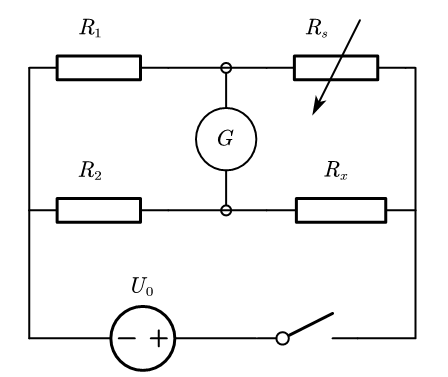
\includegraphics[width=\textwidth]{figures/自绘电桥.png}
        \caption{惠斯登电桥示意图}
        \label{fig:a}
    \end{subfigure}
    \begin{subfigure}[b]{0.415\textwidth}
        \centering
        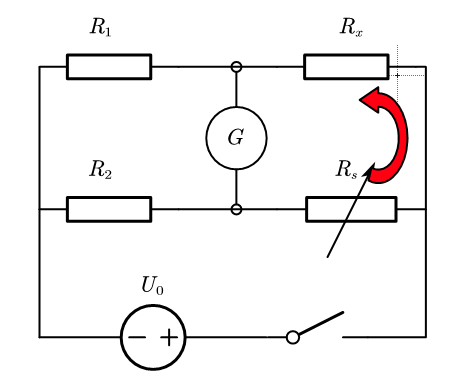
\includegraphics[width=\textwidth]{figures/交换法.png}
        \caption{交换法测量示意图}
        \label{fig:b}
    \end{subfigure}
    \caption{惠斯登电桥相关示意图}
    \label{fig:fig1}
\end{figure}


\begin{enumerate}[label=(\arabic*)]
\item \textbf{直接法}

如图\ref{fig:a}所示,$R_1,R_2$为已知电阻,$R_s$为电阻箱,$R_x$为待测电阻,$E$为电源,$G$为检流计。点$A,B$分别为电桥的两个中点。
根据图中已知电阻$R_1,R_2$、电阻箱$R_s$和待测电阻$R_x$,我们可以计算得到检流计上下两端的电势差为:
\begin{equation}
    U=V_A-V_B=\Big(\frac{R_2}{R_1+R_2}-\frac{R_x}{R_s+R_x}\Big)E
\end{equation}

当电桥平衡时,$U=0$,即$V_A=V_B$,此时有:
\begin{equation}
    \frac{R_2}{R_1+R_2}=\frac{R_x}{R_s+R_x}
\end{equation}

解出待测电阻$R_x$:
\begin{equation}
    R_x=\frac{R_2}{R_1}\cdot R_s
\end{equation}

在实际测量中,通常通过调节电阻箱$R_s$的值,使得检流计的指针指向零点,从而实现电桥的平衡状态。通过读出已知电阻$R_1,R_2$和电阻箱$R_s$的值,可以计算出待测电阻$R_x$的值。

\item \textbf{交换法}

在原有直接法的基础上,如图\ref{fig:b}所示,我们将待测电阻$R_x$与电阻箱$R_s$的位置互换,重新调节电阻箱得到测量电阻$R_s'$,使得检流计的指针再次指向零点,从而实现电桥的平衡状态。
通过测量已知电阻$R_1,R_2$和电阻箱$R_s'$的值,可以计算出待测电阻$R_x$的值:

两次平衡条件分别为(第一次为直接法配置,第二次为交换后配置):
\begin{equation}
R_x=\frac{R_2}{R_1}R_s,\quad
R_x=\frac{R_1}{R_2}R_s'.
\end{equation}
两式相乘得
\begin{equation}
\overline{R_x}^2=R_sR_s'\quad\Rightarrow\quad \overline{R_x}=\sqrt{R_sR_s'}.
\end{equation}
所以,交换法测得的待测电阻$R_x$为两次测量结果的几何平均值$\overline{R_x}=\sqrt{R_sR_s'}$
\end{enumerate}

\subsubsection{误差分析}

\begin{enumerate}[label=(\arabic*)]

\item \textbf{不确定度的主要来源}

惠斯登电桥测量的不确定度主要来源于系统误差(B类不确定度),其可能的来源有以下几种:

    \paragraph{电阻箱的固有误差}
    标准电阻箱 ($R_s$) 自身存在误差,其示值与真实值之间存在偏差。该误差属于B类不确定度,电阻箱的相对误差可表示为:
    \begin{equation}
    \frac{\Delta R_s}{R_s} \approx C_1 + \frac{C_2 \cdot m}{R_s}
    \end{equation}
    其中 $C_1, C_2$ 是与电阻箱精度等级相关的常数,$m$ 是所用旋钮的个数。在本次实验当中,$C_1=0.001$,$C_2=0.002,m=6$。该误差是不可避免的系统误差的主要来源。
    \paragraph{电桥灵敏度限制}
    检流计的灵敏度是有限的。当电桥接近平衡时,微小的电阻变化可能无法引起检流计指针的明显偏转。我们将人眼能察觉的最小偏转(如0.2分格)定义为观测阈值,而根据这一阈值我们定义了电桥灵敏度。电桥灵敏度 $S$ 定义为单位相对电阻变化引起的偏转格数,即:
    \begin{equation}
        S = \frac{\Delta d}{\Delta R_s / R_s}
    \end{equation}
    其中 $\Delta d$ 为变动相对单位电阻后引起的偏转格数,此处的$\Delta R_s$和上文的不同,是指电阻箱的一个微小变动量。根据这一数值,我们便可以计算出,当指针移动0.2分格时,电阻箱的相对变动量为 
    \begin{equation}
        \frac{\Delta R_s}{R_s} = \frac{\Delta d}{S}
    \end{equation}
    由于我们将0.2分格作为观测阈值,因此当指针移动0.2分格时,电阻箱的相对变动量为 $\frac{\Delta R_s}{R_s}=\frac{0.2}{S}$。因此,由检流计灵敏度限制引入的相对不确定度分量为 $\frac{0.2}{S}$。
    \paragraph{比率臂的系统误差}
    比率臂电阻 $R_1$ 和 $R_2$ 也存在固有误差。在直接法测量中($R_x = \frac{R_1}{R_2}R_s$),这两个电阻的误差会直接传播到最终结果中,成为一个不可忽略的系统误差来源。同时,比率臂的选取,对于最终实验结果的精度也有显著影响。通常,让$R_1$和$R_2$尽可能接近,可以减小由比率臂误差引入的系统误差。

\newpage
\item \textbf{误差的控制与最终计算}

    \paragraph{交换法的作用}
    为了消除比率臂 $R_1, R_2$ 带来的系统误差,本实验采用交换法。通过交换 $R_x$ 与 $R_s$ 的位置进行两次独立测量,并对结果取几何平均值,可以大大降低比率臂 $\frac{R_1}{R_2}$ 的误差对最终结果的影响。因此,交换法可以有效提高测量的准确性。

    \paragraph{最终不确定度评估}
    采用交换法后,总不确定度主要由电阻箱的固有误差和两次测量中的灵敏度限制共同决定。最终的相对不确定度 $E$ 可由下式计算:
    \begin{equation}
    E = \frac{\Delta R_x}{R_x} = \sqrt{\left(\frac{\Delta R_s}{R_s}\right)^2 + \left(\frac{0.2}{S}\right)^2 + \left(\frac{0.2}{S'}\right)^2}=\sqrt{\left(C_1 + \frac{C_2 \cdot m}{R_s}\right)^2 + \left(\frac{0.2}{S}\right)^2 + \left(\frac{0.2}{S'}\right)^2}
    \end{equation}
    其中,第一项为电阻箱的固有误差;第二、三项分别为两次平衡测量中由电桥灵敏度 $S$ 和 $S'$ 引入的不确定度分量。
    计算出相对不确定度 $E$ 后,即可得到待测电阻的绝对不确定度 $\Delta R_x = E \cdot \overline{R}_x$,最终测量结果表示为:
    \begin{equation}
    \boxed{R_x = \overline{R}_x \pm \Delta R_x}
    \end{equation}

\end{enumerate}

\subsubsection{实验内容}
\textbf{1、自组电桥测未知电阻}

\begin{enumerate}[label=\textbf{Step}\arabic*,leftmargin=6em]    
    \item 自组电桥,选择检流计灵敏度,并将检流计"调零";
    \item 选取适当比率臂,利用交换法测量待测电阻;
    \item 测算自组电桥的灵敏度。
\end{enumerate}

\textbf{2. 用盒式惠斯登电桥测电阻离散度}
\begin{enumerate}[label=\textbf{Step}\arabic*,leftmargin=6em]
    \item 打开盒式电桥,选择工作电源,将指针调零;
    \item 选取合适的比率臂,依次测量待测电阻盘上8个等值电阻;
    \item 计算这批电阻的离散度。
\end{enumerate}

\subsection{实验重点}
\begin{enumerate}[label=(\arabic*),leftmargin=3em]
    \item 掌握惠斯登电桥工作原理及其特点,学会自组电桥测量未知电阻;
    \item 理解不确定性和误差分析的方法和技巧;
    \item 掌握正确使用盒式惠斯登电桥测量电阻的方法;
\end{enumerate}
\subsection{实验难点}
\begin{enumerate}[label=(\arabic*),leftmargin=3em]
    \item 熟练组装和使用惠斯登电桥;
    \item 掌握不确定度和误差分析的方法;
\end{enumerate}

\begin{fullreportonly}
\section{原始数据(20分)}
\begin{figure}[H]
    \centering
    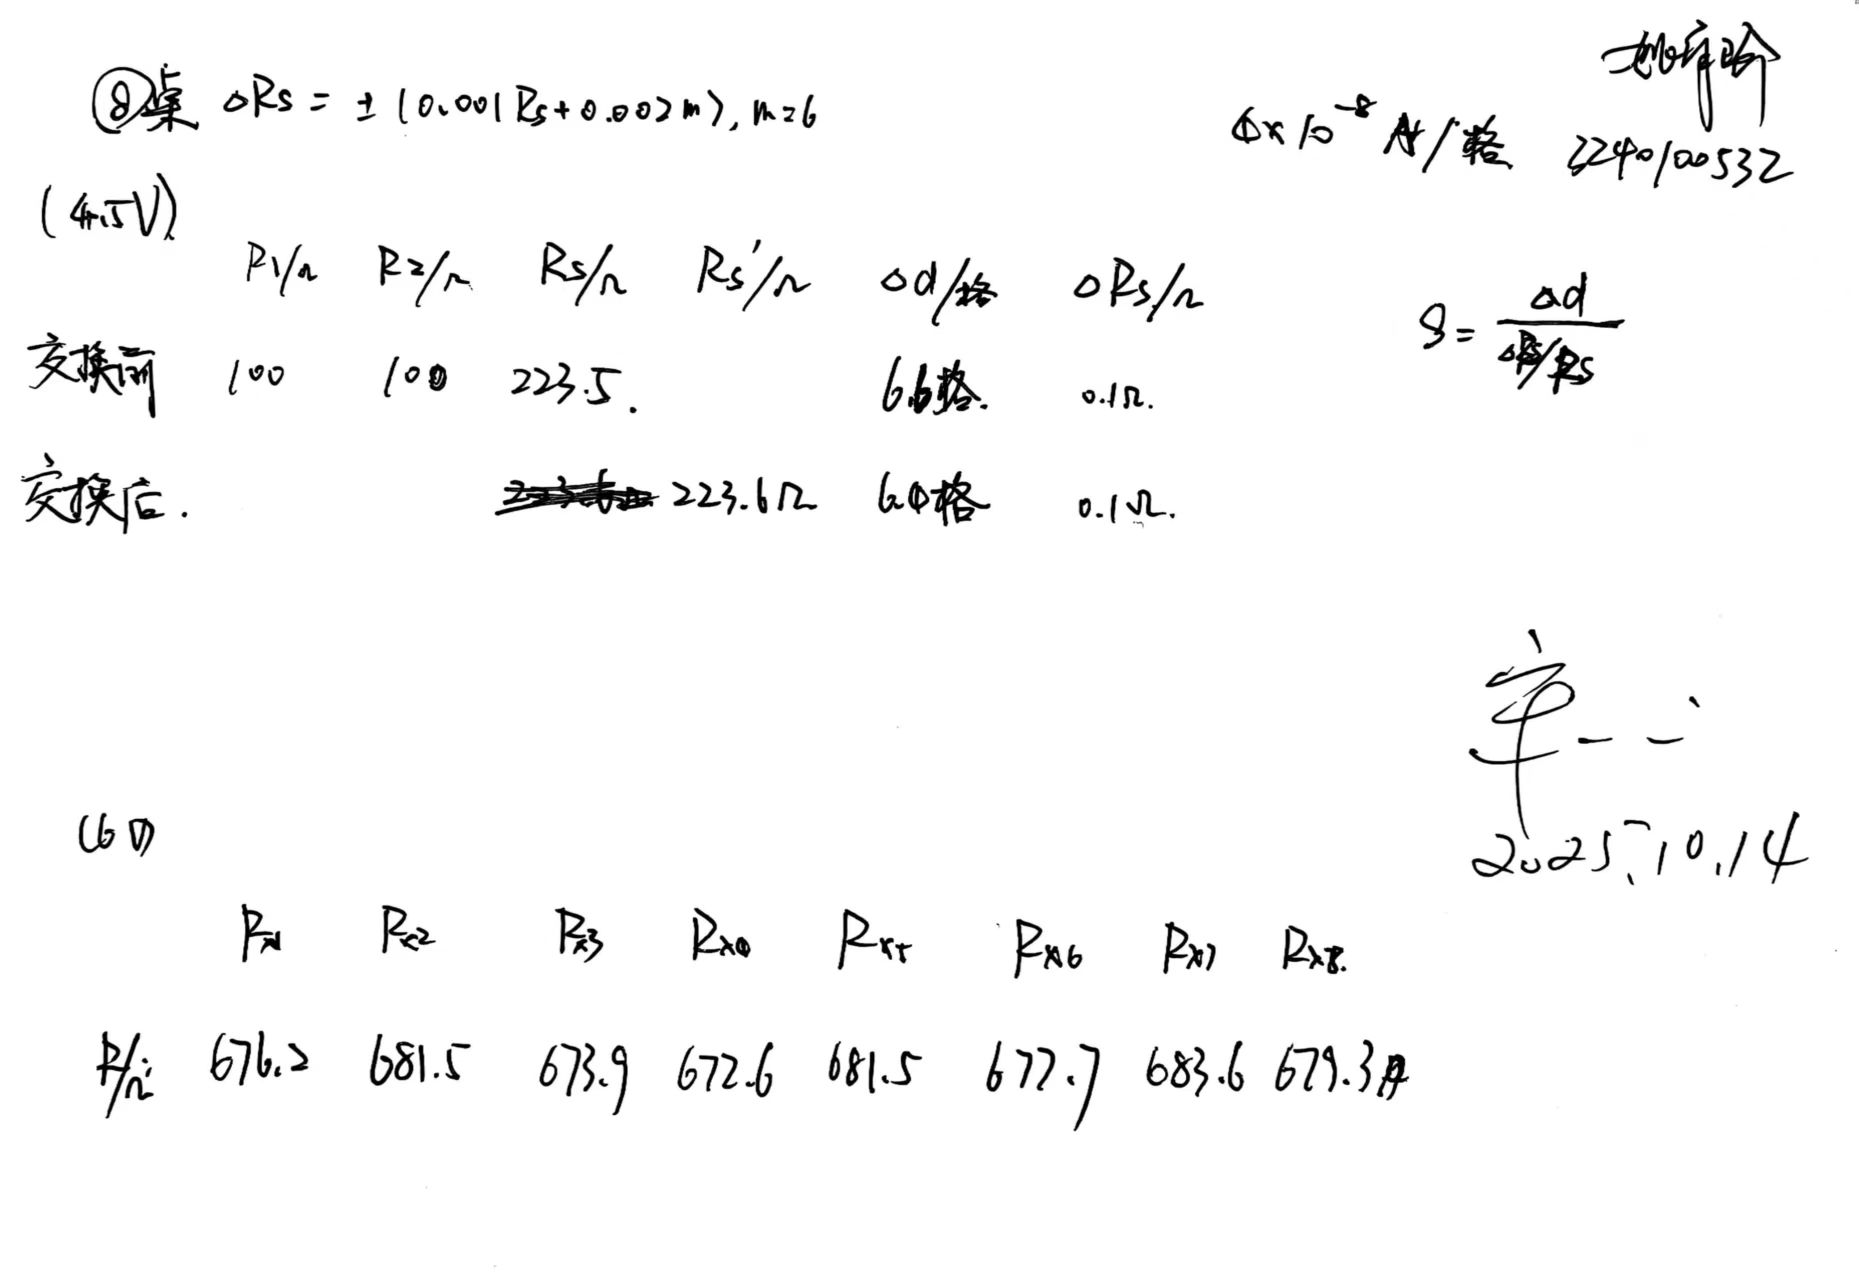
\includegraphics[width=0.7\textwidth]{figures/原始数据.jpg}
    \caption{原始数据记录}
    \label{fig:fig2}
\end{figure}

\section{结果与分析(60分)}
\subsection{数据处理与结果(30分)}
下表给出交换前后电桥平衡时的关键读数与由电桥灵敏度计算所需要的一些量:
\begin{table}[H]
\centering
\caption{交换前后平衡读数与可分辨改变量}
\begin{tabularx}{0.8\textwidth}{|c|*{7}{>{\centering\arraybackslash}X|}}
\hline
 & $R_1/\Omega$ & $R_2/\Omega$ & $R_s/\Omega$ & $R_s'/\Omega$ & $\Delta d$/格 & $\Delta R_s/\Omega$ \\
\hline
交换前 & 100 & 100 & 223.5 & --- & 6.6 & 0.1 \\
\hline
交换后 & 100 & 100 & --- & 223.6 & 6.4 & 0.1 \\
\hline
\end{tabularx}
\label{tab:exchange}
\end{table}
根据表\ref{tab:exchange}中的数据,利用交换法计算待测电阻$R_x$的值:
    \begin{equation}
        \overline{R_x} = \sqrt{R_s R_s'} = \sqrt{223.5 \times 223.6} \approx 223.55\,\Omega
    \end{equation}

下表给出利用盒式电桥测量得到的8个电阻的读数:
% 让每列宽度均分,数据占满0.8\textwidth
\begin{table}[H]
\centering
\caption{各电阻测量值}
\begin{tabularx}{0.8\textwidth}{|c|*{8}{>{\centering\arraybackslash}X|}}
\hline
电阻 & $R_1/\Omega$ & $R_2/\Omega$ & $R_3/\Omega$ & $R_4/\Omega$ & $R_5/\Omega$ & $R_6/\Omega$ & $R_7/\Omega$ & $R_8/\Omega$ \\
\hline
电阻值 & 676.2 & 681.5 & 673.9 & 672.6 & 681.5 & 677.7 & 683.6 & 679.3 \\
\hline
\end{tabularx}
\label{tab:resistors}
\end{table}
可以根据表\ref{tab:resistors}中的数据,画出电阻分布图如下:
\begin{figure}[H]
    \centering
    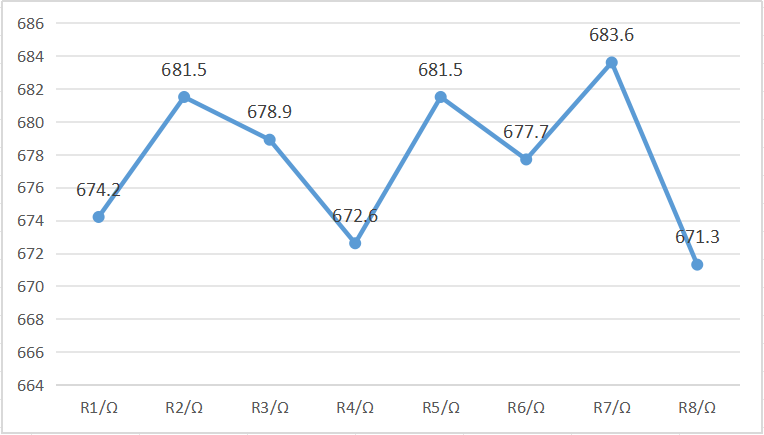
\includegraphics[width=0.6\textwidth]{figures/电阻测量值.png}
    \caption{电阻测量值分布图}
    \label{fig:resistor_distribution}
\end{figure}

计算出8个电阻的平均值:
\begin{equation}
    \overline{R} = \frac{1}{8} (676.2 + 681.5 + 673.9 + 672.6 + 681.5 + 677.7 + 683.6 + 679.3) = \frac{5426.3}{8} \approx 678.29\,\Omega
\end{equation}


\subsection{误差分析(20分)}

\subsubsection{自组电桥测量实验误差}
\begin{enumerate}
    \item 计算电阻箱的固有误差
    
    由表\ref{tab:exchange}中的数据,电阻箱$R_s=223.5\,\Omega$,旋钮个数$m=6$,代入公式计算电阻箱的相对误差:
    \begin{equation}
        \frac{\Delta R_s}{R_s} \approx C_1 + \frac{C_2 \cdot m}{R_s} = 0.001 + \frac{0.002 \cdot 6}{223.5} \approx 0.001054
    \end{equation}

    \item 计算电桥灵敏度
    
    根据表\ref{tab:exchange}中的数据,交换前后电桥灵敏度分别为:
    \begin{align*}
        S &= \frac{\Delta d}{\Delta R_s / R_s} = \frac{6.6}{0.1 / 223.5} \approx 14751 \\
        S' &= \frac{\Delta d}{\Delta R_s / R_s} = \frac{6.4}{0.1 / 223.6} \approx 14310
    \end{align*}

    \item 计算最终不确定度
        
    根据上述两个计算结果,可以综合计算得到相对不确定度$E$:
    \begin{align*}
        E &= \sqrt{\left(\frac{\Delta R_s}{R_s}\right)^2 + \left(\frac{0.2}{S}\right)^2 + \left(\frac{0.2}{S'}\right)^2} \\
          &\approx \sqrt{(0.001054)^2 + \left(\frac{0.2}{14751}\right)^2 + \left(\frac{0.2}{14310}\right)^2} \\
          &\approx \sqrt{(0.001054)^2 + (1.357 \times 10^{-5})^2 + (1.398 \times 10^{-5})^2} \\
          &\approx 0.001054
    \end{align*}
    
    计算绝对不确定度$\Delta R_x$:
    \begin{equation}
        \Delta R_x = E \cdot \overline{R_x} = 0.001054 \times 223.55 \approx 0.23\,\Omega
    \end{equation}

\end{enumerate}    
因此,待测电阻的最终结果为:
    \begin{equation}
        \boxed{R_x = 223.55 \pm 0.23\,\Omega}
    \end{equation}

\subsubsection{盒式电桥测量实验误差}
    
\begin{enumerate}
    \item 计算标准差
    
根据表\ref{tab:resistors}中的数据,计算8个电阻的标准差$S$:
\begin{align*}
    S &= \sqrt{\frac{1}{N-1} \sum_{i=1}^{N} (R_i - \overline{R})^2} \\
      &\approx \sqrt{\frac{106.43}{7}} \approx \sqrt{15.20} \approx 3.90\,\Omega
\end{align*}

    \item 计算离散度

离散度$\alpha$定义为标准差与平均值的比值,表示为:
\begin{equation}
    \alpha = \frac{S}{\overline{R}} \times 100\% \approx \frac{3.90}{678.29} \times 100\% \approx 0.57\%
\end{equation}

\end{enumerate} 

\subsubsection{误差结果分析}
通过上述计算,我们得到了自组电桥测量的待测电阻$R_x = 223.55 \pm 0.23\,\Omega$,这一结果表明测量具有较高的精度,误差控制在0.1\%以内,符合实验预期。同时,盒式电桥测量的8个电阻的离散度约为0.57\%,显示出这些电阻的一致性较好。总体来看,实验结果可靠,误差分析合理。


\subsection{实验探讨(10分)}
在本次实验中,我们通过自组电桥和盒式惠斯登电桥两种方法测量了电阻,并对测量结果进行了误差分析。在理论层面,我理解了惠斯登电桥的工作原理及其在精确测量中的应用。同时,我也学会了系统的误差分析方法,如识别误差来源、计算不确定度等;
在实践层面,我掌握了组装和调试惠斯登电桥的技能,学会了如何通过调节电阻箱实现电桥平衡,同时也学会了盒式电桥快速测量电阻的方法。

\section{思考题(10分)}
\subsection{为何用惠斯登电桥测电阻比伏安法测量准确度高?电桥法测电阻产生误差的主要因素是什么?}

\subsubsection{电桥法测量准确高的原因}
\begin{enumerate}
    \item \textbf{减少系统误差:}惠斯登电桥通过平衡电桥的方式测量电阻,避免了直接测量电流和电压时可能引入的系统误差,如电流表和电压表的内阻影响。
    \item \textbf{灵敏度高:}电桥法可以通过调节比率臂和标准电阻,使检流计指针灵敏地反映微小的电阻变化,测量分辨率高。
    \item \textbf{受外界干扰小:}电桥平衡时,桥路中电流极小,测量结果不易受电源电压波动等外界因素影响。
\end{enumerate}
\subsubsection{用电桥法测电阻产生误差的主要因素}
\begin{enumerate}
    \item \textbf{桥臂电阻的误差:}测量结果$ R_x = \frac{R_1}{R_2} \cdot Rs $的精度直接依赖于三个已知电阻$R_1, R_2, R_s$的精度。如果这些电阻的标值不准确,或因温度变化而改变,都会直接导致系统误差。
    \item \textbf{电桥的灵敏度带来的误差:}如果电桥灵敏度不够高,当检流计指针指在“零”位时,
        桥路可能并未完全平衡,只是失衡电流太小以至于检流计无法检测到。这个无法被察
        觉的微小失衡就会带来误差。
\end{enumerate}

\subsection{为了提高电桥测量灵敏度,应采取哪些措施?为什么?}
\subsubsection{具体措施}
\begin{enumerate}
    \item 在一定程度内增大电源电压,可增加桥路中的电流,从而放大检流计的响应信号。
    \item 使比率臂$\frac{R_1}{R_2}$的取值接近1,此时电桥对电阻变化的灵敏度最高。
    \item 选用分度值更小的电阻箱,可以得到更多有效数字,也更容易让电桥严格平衡。
\end{enumerate}
\subsubsection{原因}
增大电源电压可以提高桥路中的电流,使检流计对微小电阻变化更敏感,从而提升测量分辨率。比率臂接近1时,电桥对待测电阻的变化响应最大,灵敏度最高,有助于更准确地判别平衡状态。因此,这两项措施都能有效提高电桥测量的灵敏度和准确性。

\subsection{用电桥测电阻时,若线路接通后检流计指针总是往一个方向偏转或总不偏转,试分析是什么原因?}
\subsubsection{总是往一个方向偏转}
可能是因为比率臂选择不合适,导致标准电阻$R_s$的调节范围无法覆盖被测电阻$R_x$,使电桥始终无法达到平衡。此外,也可能是电路连接错误,导致电流始终流向一个方向。
\subsubsection{总不偏转}
如果检流计指针始终不偏转,可能是电路某处断开,如导线、开关等损坏,或电源未接通。也可能是检流计本身故障或被短路,导致无法显示电流变化。

\subsection{惠斯登电桥比率臂选取的原则是什么?为什么要这样选取?}
\subsubsection{原则}
\begin{enumerate}
    \item 使标准电阻$R_s$的调节范围覆盖被测电阻;
    \item 尽量使比率臂接近1;
    \item 使用的确定电阻阻值尽可能和待测电阻差不多大。
\end{enumerate}
\subsubsection{原因}
合理选取比率臂可以确保$R_s$的调节范围覆盖待测电阻$R_x$,避免因量程不足而无法实现电桥平衡。同时,比率臂接近1时,电桥的灵敏度最高,有助于提高测量的准确性和分辨率,减小由比率臂误差带来的影响。
而确定电阻与待测电阻阻值相近,可以使电桥在平衡时的调节更为灵敏,减少因电阻差异过大而引起的测量误差。
\subsection{如何使用自组电桥测量电表内阻(注意电表所能允许通过的最大电流)?根据电桥平衡的特点,可否将桥路中的检流计去掉,换成行测电表判别电桥的平衡?}

\subsubsection{测量方法}
    \begin{enumerate}
      \item 接法:将被测电表串联一个保护电阻 $R_p$,共同接入电桥的待测电阻位置(图\ref{fig:a}中$R_x$位置)。
      \item 限流:设电源两端电压 $U$ ,最大允许电流 $I_g$ ,电表内阻$R_g$,则保护电阻需满足
      $ R_p \ge \frac{U}{I_g} - R_g$
      \item 操作与求值:先置大 $R_p$ 与较大 $R_s$,缓慢上电,调 $R_s$(必要时微调比率臂)至电表示零(电表两端电势差近零)。平衡时
      \[
        R_g = R_x- R_p = \frac{R_1}{R_2}\,R_s- R_p.
      \]
    \end{enumerate}

\subsubsection{检流计可否用行测电表替代?}
    原则上可以:平衡时读数电表读数也会趋近零,按照原理也可以使用。但不推荐,因为:
    \begin{enumerate}
      \item 行测电表灵敏度过低,难以准确判断电桥平衡状态;
      \item 行测电表内阻较大,可能更容易影响电桥的平衡;
    \end{enumerate}

\end{fullreportonly}
\insertnotes
\end{document}